
\documentclass[12pt, letter]{article}
\usepackage[utf8]{inputenc}
\usepackage[spanish,es-tabla]{babel}
%\usepackage{times},puede ser arial 
\usepackage{csquotes}
\usepackage[left=2.54cm, right=2.54cm,top=2.54cm,bottom=2.54cm]{geometry}
\renewcommand{\baselinestretch}{1.5}
\usepackage[backend=biber,style=apa]{biblatex}
\bibliography{Referencias.bib}
\usepackage{graphicx}
\usepackage{subcaption}
\usepackage[hidelinks]{hyperref}

\title{\huge{Interrupciones}}
\author{Victor Manuel Arbeláez Ramírez \\ Facultad de ingeniería \\ Universidad de Antioquia}
\date{}

\begin{document}\raggedright

\maketitle


\section*{Introducción}
Los microprocesadores son herramientas que pueden ejecutar una gran cantidad de instrucciones en un segundo, por lo que, para hacer uso del mayor potencial de sus capacidades, se opta eficientemente por las ventajas que deja el sistema de las interrupciones como se podrá apreciar a continuación. Aun así, el concepto de éstas interrupciones es un poco más complejo de entender, debido a que es poco intuitivo con respecto a lo que se viene aprendiendo en los cursos básicos de computación y programación, en donde la mayoría de procesos se ejecuta de una manera continua. Se enunciará entonces, su definición, su historia, los tipos que existen y la forma de implementarlos teniendo como objetivo el conocer que son y para que se usan las interrupciones a nivel del microprocesador.
\newpage

\section*{¿Qué es una interrupción en el contexto de los microprocesadores?}

\setlength{\parindent}{31pt}
Una definición para el concepto de interrupción podría ser: Una interrupción consiste en un mecanismo que provoca la alteración del orden lógico de ejecución de instrucciones como respuesta a un evento externo, generado por el hardware de entrada/salida en forma asincrónica al programa que está siendo ejecutado y fuera de su control. 

\setlength{\parindent}{31pt}
Como se expresa en la definición una interrupción es un mecanismo que altera la secuencia lógica de ejecución, por lo que la próxima instrucción a ejecutarse no es la que se tenía prevista inicialmente en el del orden lógico, sino que se pasa a la primera instrucción de otro servicio o proceso causante de la interrupción.

\setlength{\parindent}{31pt}
El programa de interrupción es semejante a una subrutina, ya que debe almacenar los datos de estado y registro y conservar el contenido del microprocesador antes de la interrupción.

\section*{¿Se puede hablar de la historia de las interrupciones?}

\setlength{\parindent}{31pt}
No se puede hablar propiamente de la historia de las interrupciones, pero se sabe que están presentes desde la invención de los controladores basados en la arquitectura de von Neumann y los microcontroladores, ya que había la necesidad de interactuar con los periféricos externos, pero no de forma mecánica, sino mediante un software provisto de instrucciones al procesador. Inicialmente, la técnica que se empleo fue que el propio controlador se encargase de sondear el dispositivo cada cierta cantidad de tiempo "polling" para conocer en qué momento ejecutar la interrupción. Después, para desentenderse de ésta problemática se optó propiamente por los conceptos de interrupciones, en donde se delega la responsabilidad al periférico para que avise de la necesidad de "interrumpir" un proceso y  así evitar el estar sondeando cada cierto tiempo.

\section*{¿Qué tipo de interrupciones existen?}

\setlength{\parindent}{31pt}
En general sobre el tipo de interrupciones, existen las internas y externas.

\setlength{\parindent}{31pt}
Una interrupción externa es aquella que proviene de un dispositivo E/S (entrada / salida) y una interrupción interna es una compuerta de estado o un señalamiento dentro del microprocesador que pueden ser activados o desactivados mediante instrucciones de interrupción especiales. 

\setlength{\parindent}{31pt}
Generalmente, cuando se desactiva una interrupción interna, el microprocesador no da servicio a interrupciones externas. Contrariamente si se activa la interrupción interna, el sistema puede responder a interrupciones externas. Cuando se atiende a una interrupción, lo primero que el microprocesador hace, es desactivar las interrupciones internas para evitar atender otras interrupciones.

\setlength{\parindent}{31pt}
Se presenta otro tipo de interrupciones, pero solo en algunos microprocesadores, los cuales cuentan con líneas de interrupción no enmascarables mediante las cuales se hace caso omiso del estado de la compuerta de interrupción interna y se siguen aceptando interrupciones.

\begin{figure}[h!] %invoca una figura con el parámetro here
    \raggedright
        \begin{subfigure}[b]{0.45\linewidth}
            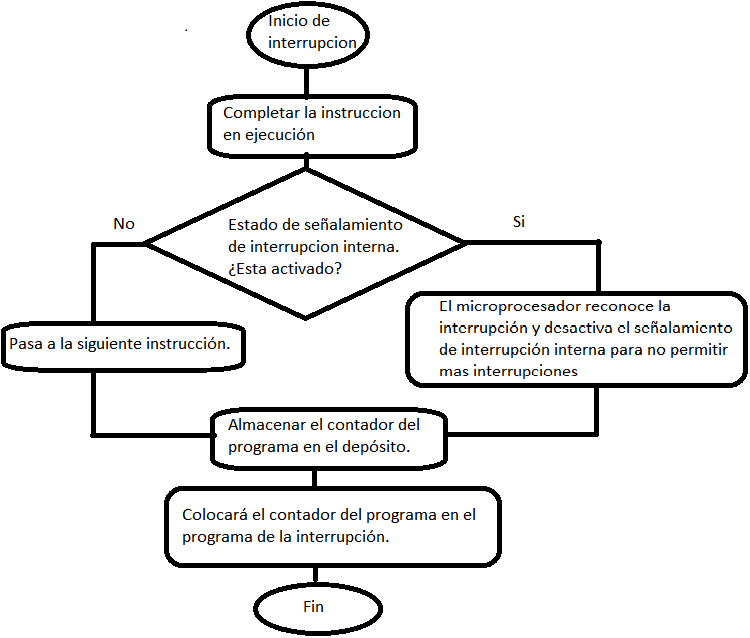
\includegraphics[width=\linewidth]{Figuras/diagrama1.png}
            \caption{Comunicación típica del microprocesador}
            \label{fig:diagrama1}
        \end{subfigure}
    \raggedleft
        \begin{subfigure}[b]{0.45\linewidth}
            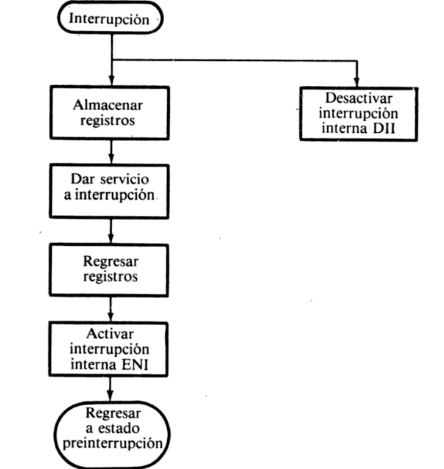
\includegraphics[width=\linewidth]{Figuras/diagrama2.png}
            \caption{Secuencia del programa de interrupción}
            \label{fig:diagrama2}
        \end{subfigure}
    \caption{Diagramas de interrupciones}
    \label{fig:Diagramas}
\end{figure}

\setlength{\parindent}{31pt}
Normalmente en una comunicación con el microprocesador, responderá como se muestra  en la Figura ~\ref{fig:diagrama1}.

\setlength{\parindent}{31pt}
Se presentan también interrupciones múltiples, en donde los dispositivos de micro procesamiento, generalmente están limitados en cuanto al número de conexiones y en ocasiones cuentan con algunas conexiones de señales dedicados para interrupciones. Cuando se requiere que una gran cantidad de dispositivos E/S, se interrelacionen con el sistema de micro procesamiento, las líneas de solicitud de estos dispositivos se someten a una operación “o” lógica, tal como se muestra en la Figura ~\ref{fig:diagrama2}.

\section*{¿Cómo se hace la implementación de interrupciones a nivel de hardware?}

\setlength{\parindent}{31pt}
Una interrupción por hardware es un mecanismo de comunicación entre el procesador y los dispositivos de E/S. Sirve para indicar que un dispositivo de E/S tiene datos pendientes de ser tratados. Las interrupciones por hardware evitan que el sistema operativo tenga que muestrear periódicamente el estado de los dispositivos de E/S, de manera que son ellos mismos los que indican que hay datos para ser tratados. \parencite{Int_Ex}.

\setlength{\parindent}{31pt}
 El agente generador o solicitante de la interrupción activa la mencionada señal cuando necesita que se le atienda, es decir, que se ejecute un programa que le atienda. \parencite{Micro} Ante la solicitud de una interrupción, siempre y cuando esté habilitado ese tipo de interrupción, la unidad de control realiza un ciclo de aceptación de interrupción. 
 
 \section*{ ¿Cómo se implementan las interrupciones por software?}

\setlength{\parindent}{31pt}
Una interrupción por software es un mecanismo de comunicación entre un proceso (que se ejecuta en modo usuario) y el sistema operativo (que se ejecuta en modo supervisor). El proceso emplea las interrupciones por software para notificar al sistema operativo que requiere de su intervención. En procesadores x86, para lanzar una interrupción por software un proceso ejecuta la instrucción int seguida de un número de 16 bits que indica el tipo de interrupción por software. Por ejemplo, las llamadas al sistema en x86 se implementan mediante interrupciones por software, por medio de la instrucción int 0x80 (sin embargo, hoy día las arquitecturas de los procesadores modernos vienen con instrucciones especializadas para la invocación de llamadas al sistema como syscall en x86, por tanto, esta técnica ha caído en desuso). \parencite{Int_Ex}.

\setlength{\parindent}{31pt}
Más genéricamente aplica cuando hay múltiples controladores conectados en OR a la misma entrada de INT, sea ésta única o no. \parencite{ArquitecturaCom}. En esta situación la rutina de servicio de la interrupción debe tener una parte inicial que consista en el recorrido de los distintos controladores de E/S, leyendo los registros de estado hasta encontrar aquél que tenga su bit de "pedido de interrupción" en "1". En ese caso se invocará a la sub-rutina asociada a ese controlador específico.

\setlength{\parindent}{31pt}
Para éstos procesos de interrupciones por software, se marca una mayor eficiencia cuando se utiliza el lenguaje ensamblador o lenguaje de máquina para comunicarse directamente con el microprocesador

\printbibliography[title={Referencias}\nocite{*}]

\end{document}\raggedright
